\renewcommand{\theequation}{\theenumi}
\begin{enumerate}[label=\arabic*.,ref=\thesubsubsection.\theenumi]
\numberwithin{equation}{enumi}
%
\item Let $\triangle{ABC}$ be an equilateral triangle. Let $AB$ be the base and $\vec{M}$ be the midpoint.
\begin{enumerate}

\item $\vec{A} = \myvec{0\\m}$ (as point $\vec{A}$ lies on the y-axis) \\
$\vec{B} = \myvec{0\\n}$ (as point $\vec{B}$ lies on the y-axis) \\
$\vec{M} = \myvec{0\\0}$ (as point $\vec{M}$ lies on the origin) \\
$\vec{C} = \myvec{p\\0}$ (as point $\vec{A}$ lies on the x-axis) 
\\

$\norm{\vec{A}-\vec{B}} = \norm{\vec{B}-\vec{C}} = \norm{\vec{C}-\vec{A}} = 2a$

\item $\vec{M}$ is the mid-point of $\vec{A}$ and $\vec{B}$ \\
$\vec{M} = \frac{\vec{A}+\vec{B}}{2}$ \\
$\implies m = -n$  \\
$\norm{\vec{A}-\vec{B}} = 2a$ \\ 
$\implies m = -n = a$ \\


\item $\norm{\vec{C}-\vec{A}} = 2a$ \\
$\sqrt{p^2+a^2} = 2a$
$\implies p = \pm\sqrt{3}a$\\


\item The vertices are, \\
$\vec{A} = \myvec{0\\a}$  \\
$\vec{B} = \myvec{0\\-a}$ \\
$\vec{C} = \myvec{\pm\sqrt{3}a\\0}$

$\triangle{ABC}$ in Fig.\ref{fig:tri_1}  is generated using the following python code
\begin{lstlisting}
codes/line/miscellaneous/tri_equi.py
\end{lstlisting}
\begin{figure}[!ht]
\centering
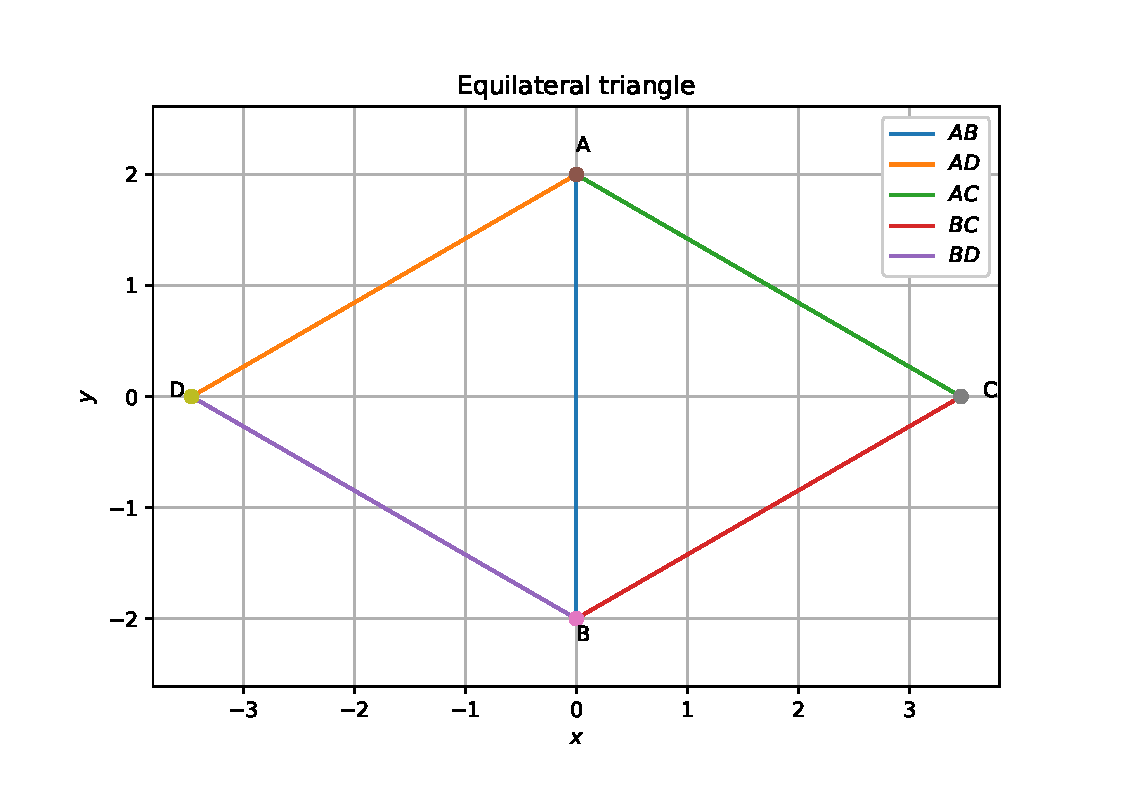
\includegraphics[width=\columnwidth]{./codes/line/miscellaneous/tri_equi.eps}
\caption{Triangles $ABC$ and $ABD$ using python}
\label{fig:tri_1}
\end{figure} 

\end{enumerate}

\end{enumerate}
